\documentclass[usenames,dvipsnames,notes,11pt,aspectratio=169]{beamer}
\usepackage{ifthen}
\usepackage{xcolor}
\usepackage{pgfplots}
\usepackage{amsmath}
\usepackage{centernot}
\usepackage{pifont}
\usepackage{tabularx}
\usepackage{makecell}
\usepackage{cuted}
\usepackage{booktabs}
\usepackage{array}
\usepackage{textcomp}
\usepackage{setspace}
\usepackage{xspace}
\usepackage{tikz}
\usepackage{pdfcomment}
%\newcommand{\pdfnote}[1]{\marginnote{\pdfcomment[icon=note]{#1}}}
\newcommand{\pdfnote}[1]{}

\usepackage{pgfpages}
%\setbeameroption{show notes on second screen}


\input ../beamer-style
\input ../std-macros
\input ../macros

\AtBeginSection[]
{
    \begin{frame}
        \frametitle{Table of Contents}
        \tableofcontents[currentsection]
    \end{frame}
}
\parskip=10pt

\title[CSCI-GA.2590]{Distributed representation of text}
\author[He He]{He He
}
\institute[NYU]{
    
\includegraphics[height=1cm]{../figures/nyu-logo}\\
}
\date{January 31, 2023}

\begin{document}
\begin{frame}
\titlepage
\end{frame}

\begin{frame}
    {Logistics}
    \begin{itemize}
        \item HW1 released. Due by next Friday. 
        \item Plan for today:
            \begin{itemize}
                \item Lecture: 75 minutes
                \item Break: 5 minutes
                \item Section by Nitish: 40 minutes
            \end{itemize}
    \end{itemize}
\end{frame}

\section{Review}
\begin{frame}
    {Last week}
    Generative vs discriminative models for text classification\\
    \begin{itemize}
        \item (Multinomial) naive Bayes \hfill What's the key assumption?
            \pause
            \begin{itemize}
                \item Assumes conditional independence
                \item Very efficient in practice (closed-form solution)
            \end{itemize}
        \pause
        \item Logistic regression \hfill What's the main advantage?
            \pause
            \begin{itemize}
                \item Works with all kinds of features
                \item Wins with more data
            \end{itemize}
    \end{itemize}

    \pause
    Feature vector of text input\\
    \begin{itemize}
        \item BoW representation
        \item N-gram features (usually $n\le 3$)
    \end{itemize}

    \pause
    Control the complexity of the hypothesis class\\
    \begin{itemize}
        \item Feature selection
        \item Norm regularization
    \end{itemize}
\end{frame}

%\begin{frame}
%    {Evaluation}
%    \begin{itemize}
%        \itemsep3em
%        \item Accuracy
%        \item Precision
%        \item Recall 
%        \item F1
%        \item Macro vs micro average
%    \end{itemize}
%\end{frame}

\section{Introduction}

\begin{frame}
    {Objective}    
    \beamerblue{Goal}: come up with a \blue{good representation} of text\\
    \begin{itemize}[<+->]
        \item What is a representation?
            \begin{itemize}
                \item Feature map: $\phi\colon \text{text} \rightarrow \BR^d$, \eg BoW, handcrafted features
                \item ``Representation'' often refers to \blue{learned} features of the input
            \end{itemize}
        \item What is a good representation?
            \begin{itemize}
                \item Leads to \blue{good task performance} (often requires less training data)
                \item Enables \blue{a notion of distance} over text: 
                    $d(\phi(a), \phi(b))$ is small for semantically similar texts $a$ and $b$
            \end{itemize}
    \end{itemize}
\end{frame}

\begin{frame}
    {Distance functions}

    \textbf{Euclidean distance}\\
    \begin{itemize}
        \item[] For $a,b\in\BR^d$,
            $$
            d(a,b) = \sqrt{\sum_{i=1}^d(a_i-b_i)^2} \;.
            $$
            \pause
        \item[] Assume $a$ and $b$ are BoW vectors. What if $b$ repeats each sentence in $a$ twice?
            \pause ($b_i=2a_i$)
    \end{itemize}

    \pause
    \textbf{Cosine similarity}\\
    \begin{itemize}
        \item[] For $a,b\in\BR^d$,
            $$
            \text{sim}(a,b) = \frac{a\cdot b}{\norm{a}\norm{b}} = \cos\alpha
            $$
        \item[] Angle between two vectors
    \end{itemize}
\end{frame}

\begin{frame}
    {Example: information retrieval}
    Given a set of documents and a query,
    use the BoW representation and cosine similarity
    to find the most relevant document.

    What are potential problems?

    Example:\\
    \begin{itemize}
        \item[] Q: Who \textcolor{blue}{has watched} \textcolor{red}{Avatar}?
        \item[] She \textcolor{blue}{has} \textcolor{blue}{watched} the Wandering Earth.
        \item[] \textcolor{red}{Avatar} was shown here last week.
    \end{itemize}

    \pause
    \begin{itemize}
        \item Similarity may be dominated by common words
        \item Only considers the surface form (\eg do not account for synonyms)
    \end{itemize}
    
\end{frame}

\begin{frame}
    {TFIDF}
    \beamerblue{Key idea}: upweight words that carry more information about the document
    \pause

    Feature map $\phi\colon \text{document} \rightarrow \BR^{|\sV|}$

    TFIDF:\\
    $$
    \onslide<2->{
    \phi_i(d) = \underbrace{\text{count}(w_i, d)}_{\textstyle \text{term frequency}} \times 
    }
    \onslide<3->{
    \underbrace{\log \frac{\text{\# documents}}{\textstyle\text{\# documents containing $w_i$}}}_{\textstyle \text{inverse document frequency}}
    \;.
    }
    $$

    \begin{itemize}
            \onslide<2->{
        \item \textbf{Term frequency (TF)}: count of each word type in the document (same as BoW)
        }
            \onslide<3->{
        \item Reweight by \textbf{inverse document frequency (IDF)}: how \blue{specific} is the word type to any particular document 
        }
            \onslide<4->{
        \item Higher weight on \blue{frequent} words that only \blue{occur in a few documents}
        }
    \end{itemize}

\end{frame}

%\begin{frame}
%    {Justification for TFIDF}
%    Assumptions:
%    \begin{align}
%        p(d) &= \frac{1}{\text{\# of documents}} \\
%        p(d \mid w) &= \frac{1}{\text{\# documents containing $w$}}
%    \end{align}
%
%    Then, we have
%    $$
%    \text{PMI}(w; d) = \log\frac{p(d\mid w)}{p(d)} = \text{idf}(w, d) \;.
%    $$
%
%    IDF measures the association between a term/word and the document
%    \pdfnote{
%        This is a starter for today's discussion.
%        Here we try to find a document representation based on the co-occurrence statistics of the word and the document.
%        Can we generalize this idea further?
%    }
%\end{frame}

\section{Count-based word embeddings}

\begin{frame}
    {The distributional hypothesis}
    \nl{You shall know a word by the company it keeps.} (Firth, 1957)
    \pause

    Word guessing! (example from Eisenstein's book)\\
    \begin{itemize}[<+->]
        \item[] Everybody likes \textcolor{blue}{tezg\"uino}.
        \item[] We make \textcolor{blue}{tezg\"uino} out of corn.
        \item[] A bottle of \textcolor{blue}{tezg\"uino} is on the table.
        \item[] Don't have \textcolor{blue}{tezg\"uino} before you drive.
    \end{itemize}

    \onslide<+->{
    \beamerblue{Idea}: Represent a word by its neighbors.
    }
\end{frame}

\begin{frame}
    {Step 1: Choose the context}
    What are the neighbors? (What type of co-occurence are we interested in?)
    \medskip

    \begin{columns}
        \begin{column}{0.3\textwidth}
    Example:\\
    \begin{itemize}[<+->]
        \item word $\times$ document
        \item word $\times$ word
        \item person $\times$ movie
        \item note $\times$ song
    \end{itemize}
        \end{column}
        \begin{column}{0.65\textwidth}
            \onslide<1->{
                \begin{figure}
            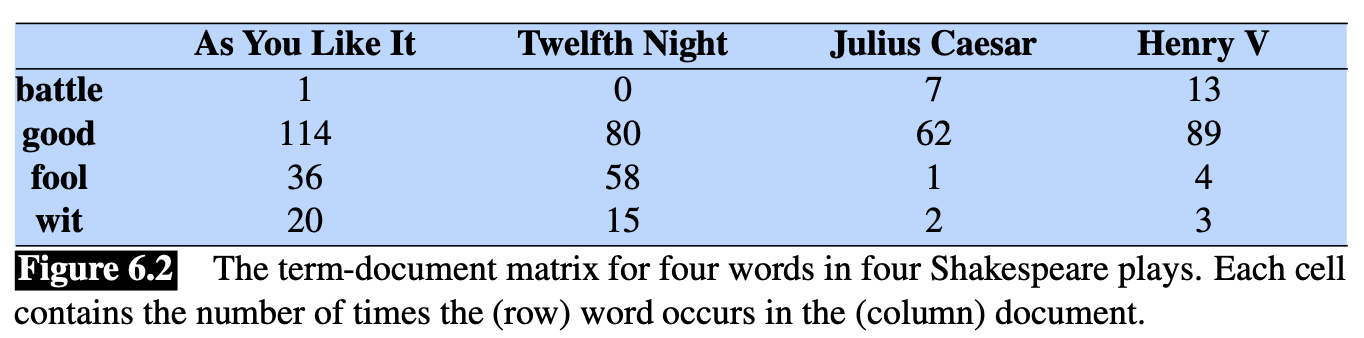
\includegraphics[width=\textwidth]{figures/term-doc-ex}
                    \caption{Jurafsky and Martin.}
                \end{figure}
            }
        \end{column}
    \end{columns}

    \medskip
    \onslide<+->{
    Construct a matrix where\\
    \begin{itemize}
        \item Row and columns represent two sets of objects
        \item Each entry is the (adjusted) co-occurence counts of the two objects
    \end{itemize}
    }

    \pdfnote{
        In the previous examples we see that the co-occurence of two words carries interesting information.
        But this is not restricted to words.
    }
\end{frame}

\begin{frame}
    {Step 2: Reweight counts}
    Upweight informative words
    \vspace{-1em}
    \begin{figure}
            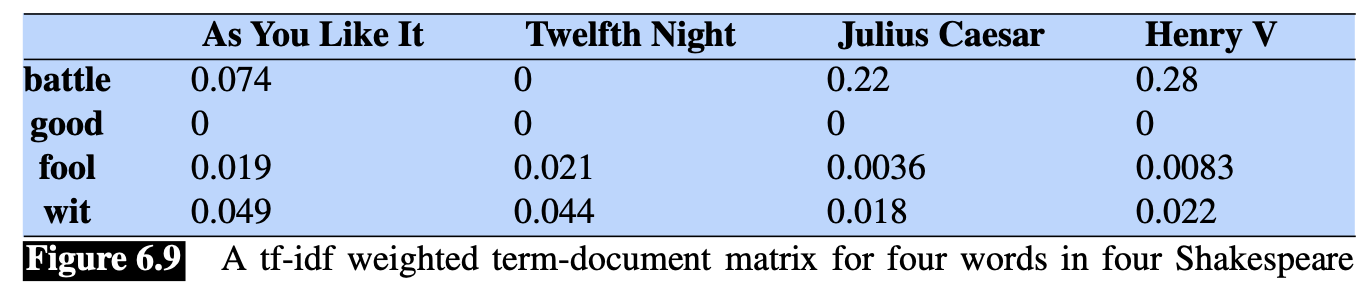
\includegraphics[width=\textwidth]{figures/term-doc-tfidf}
                    \caption{Jurafsky and Martin.}
    \end{figure}

    Each row/column gives us a word/document representation.
    
    Using cosine similarity, we can cluster documents, find synonyms, discover word meanings...
\end{frame}

\begin{frame}
    {Pointwise mutual information}
    $$
    \text{PMI}(x;y) \eqdef \log \frac{p(x,y)}{p(x)p(y)}
    = \log\frac{p(x\mid y)}{p(x)}
    = \log\frac{p(y\mid x)}{p(y)}
    $$
    \pause
    \vspace{-1em}
    \begin{itemize}
        \itemsep1em
        \item Symmetric: $\text{PMI}(x;y)=\text{PMI}(y;x)$
        \item Range: $(-\infty, \min(-\log p(x), -\log p(y)))$
        \item Estimates:
            \begin{align*}
            \hat{p}(x\mid y) = \frac{\text{count}(x,y)}{\text{count}(y)}\quad
            \hat{p}(x) = \frac{\text{count}(x)}{\sum_{x'\in\sX}\text{count}(x')}
            \end{align*}
        \item Positive PMI: $\text{PPMI}(x;y) \eqdef \max(0, \text{PMI}(x;y))$
        \item Application in NLP: measure association between words 
    \end{itemize}
\end{frame}


\begin{frame}
    {Step 3: Dimensionality reduction}
    \beamerblue{Motivation}: want a lower-dimensional, dense representation for efficiency
    \pause

    Recall \textbf{SVD}: a $m\times n$ matrix $A_{m\times n}$ (\eg a word-document matrix),
    can be decomposed to
    $$
    U_{m\times m}\Sigma_{m\times n}V_{n\times n}^T \;,
    $$
    where $U$ and $V$ are orthogonal matrices, and $\Sigma$ is a diagonal matrix.
    \pause

    \beamerblue{Interpretation}:
    $$
    AA^T = (U\Sigma V^T)(V\Sigma U^T) = U\Sigma^2 U^T \;.
    $$
    \vspace{-1em}
    \begin{itemize}
        \item $\sigma_i^2$ are eigenvalues of $AA^T$ 
        \item Connection to PCA: If columns of $A$ have zero mean (i.e. $AA^T$ is the covariance matrix), then columns of $U$ are principle components of the column space of $A$.
    \end{itemize}
\end{frame}

\begin{frame}
    {SVD for the word-document matrix}
    {[board]}

    \pause
    \begin{itemize}
        \item Run truncated SVD of the word-document matrix $A_{m\times n}$
        \item Each row of $U_{m\times k}\Sigma_k$ corresponds to a word vector of dimension $k$
        \item Each coordinate of the word vector corresponds to a cluster of documents (\eg politics, music etc.)
    \end{itemize}
\end{frame}

\begin{frame}
    {Summary}
    \textbf{Count-based word embeddings}\\
    \begin{enumerate}
        \item Design the matrix, e.g. word $\times$ document, people $\times$ movie.
        \item Reweight the raw counts, e.g. TFIDF, PMI.
        \item Reduce dimensionality by truncated SVD.
        \item Use word/person/etc. vectors in downstream tasks.
    \end{enumerate}
    
    \beamerblue{Key idea}:\\
    \begin{itemize}
        \item Represent an object by its connection to other objects.
        \item For NLP, the word meaning can be represented by the context it occurs in.
        \item Infer latent features using co-occurence statistics
    \end{itemize}
\end{frame}

\section{Prediction-based word embeddings}

\begin{frame}
    {Learning word embeddings}
    \beamerblue{Goal}: map each word to a vector in $\BR^d$ such that \textit{similar} words also have \textit{similar} word vectors.
    \vspace{1em}
    \pause

    Can we formalize this as a \blue{prediction problem}?\\
    \begin{itemize}
        \item Needs to be self-supervised since our data is unlabeled.
        %\item Minimizing the objective should allow similar words to have simliar representations.
    \end{itemize}
    \pause

    \beamerblue{Intuition}: Similar words occur in similar contexts\\
    \begin{itemize}
        \item Predict the context given a word $f\colon \text{word} \rightarrow \text{context}$
        \item Words that tend to occur in same contexts will have similar representation
    \end{itemize}
    \pdfnote{
        If we can successfully predict the context given a word, that means that words that occur in similar contexts have similar representations.
    }
\end{frame}

\begin{frame}
    {The skip-gram model}
    \beamerblue{Task}: given a word, predict its neighboring words within a window
    \begin{center}
        The \red{quick} \red{brown} \blue{fox} \red{jumps} \red{over} the lazy dog
    \end{center}

    \pause
    Assume conditional independence of the context words:
    $$
    p(\mred{w_{i-k}}, \ldots, \mred{w_{i-1}}, \mred{w_{i+1}}, \ldots, \mred{w_{i+k}} \mid \mblue{w_i}) =
    \prod_{j=i-k,j\neq i}^{i+k}p(\mred{w_j}\mid \mblue{w_i})
    $$

    \pause
    How to model $p(w_j\mid w_i)$? \pause \hspace{2em} Multiclass classification
\end{frame}

\begin{frame}
    {The skip-gram model}
    Use the softmax function to predict \red{context words} from the \blue{center word}
    \begin{align*}
        p(w_j\mid w_i) %&= \frac{\exp\pb{\mred{\theta_{w_j}}\cdot \mblue{\phi(w_i)}}}
    %{\sum_{w\in\sV} \exp\pb{\theta_{w}\cdot\phi(w_i)}} \\\pause
        &= \frac{\exp\pb{\mred{\phi_{\text{ctx}}(w_j)}\cdot \mblue{\phi_{\text{wrd}}(w_i)}}}
        {\sum_{w\in\sV} \exp\pb{\phi_{\text{ctx}}(w_j)\cdot\phi_{\text{wrd}}(w_i)}}
    \end{align*}
    %
    \pause
    \think{What's the difference from multinomial logistic regression?}
    %Classification $\rightarrow$ learning word vectors:\vspace{-1em}
    %\begin{itemize}
    %    \item $\mblue{\phi(w_i)}$: input features $\rightarrow$ context representation
    %    \item $\mred{\theta_{w_j}}$: weight vector for class $w_j$
    %        $\rightarrow$ word represenation of $w_j$
    %\end{itemize}

    \pause
    Implementation:\vspace{-1em}
    \begin{itemize}[<+->]
        \item Matrix form: $\phi\colon w \mapsto A_{d\times|\sV|}\phi_{\text{one-hot}}(w)$,
        $\phi$ can be implemented as a dictionary
        \item Learn parameters by MLE and SGD (Is the objective convex?)
        \item $\phi_{\text{wrd}}$ is taken as the word embedding
    \end{itemize}
\end{frame}

\begin{frame}
    {Negative sampling}
    Challenge in MLE: computing the normalizer is expensive (try calculate the gradient)!
    \pause

    Key idea: solve a binary classification problem instead
    \begin{center}
        Is the (word, context) pair real or fake? \\
        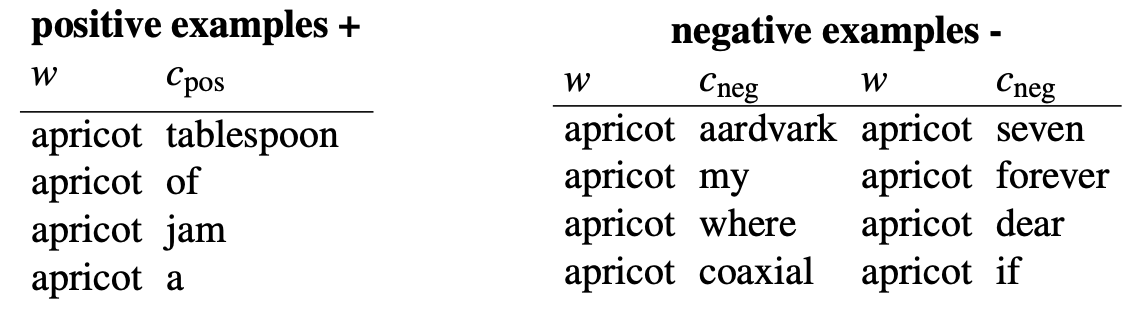
\includegraphics[height=3cm]{figures/neg-sample}
    \end{center}
    $$
    p_\theta(\text{real} \mid w, c) = \frac{1}{1+e^{-\phi_{\text{ctx}}(c)\cdot\phi_{\text{wrd}}(w)}}
    $$
\end{frame}

\begin{frame}
    {The continuous bag-of-words model}
    \beamerblue{Task}: given the context, predict the word in the middle 
    \begin{center}
        The \red{quick} \red{brown} \blue{fox} \red{jumps} \red{over} the lazy dog
    \end{center}

    Similary, we can use logistic regression for the prediction
    $$
    p(\mblue{w_i} \mid \mred{w_{i-k}}, \ldots, \mred{w_{i-1}}, \mred{w_{i+1}}, \ldots, \mred{w_{i+k}})
    $$

    How to represent the context (input)? 
\end{frame}

\begin{frame}
    {The continuous bag-of-words model}
    The context is a sequence of words.
    \begin{align*}
        c &= w_{i-k}, \ldots, w_{i-1}, w_{i+1}, \ldots, w_{i+k} \\\\
        p(w_i\mid c) &= \frac{\exp\pb{\phi_{\text{wrd}}(w_i)\cdot \phi_{\text{BoW}}(c)}}
        {\sum_{w\in\sV} \exp\pb{\phi_{\text{wrd}}(w)\cdot\phi_{\text{BoW}}(c)}} \\
        \onslide<2->{
        &= \frac{\exp\pb{\phi_{\text{wrd}}(w_i)\cdot \sum_{w'\in c}\phi_{\text{ctx}}(w')}}
        {\sum_{w\in\sV} \exp\pb{\phi_{\text{wrd}}(w)\cdot\sum_{w'\in c}\phi_{\text{ctx}}(w')}}
        }
    \end{align*}

    \onslide<2->{
    \begin{itemize}
        \item $\phi_{\text{BoW}}(c)$ sums over representations of each word in $c$
        \item Implementation is similar to the skip-gram model.
    \end{itemize}
    }
\end{frame}

\begin{frame}
    {Semantic properties of word embeddings}
        Find similar words: top-$k$ nearest neighbors using cosine similarity
            \begin{itemize}
                \item Size of window influences the type of similarity
                \item Shorter window produces \blue{syntactically similar} words, \eg Hogwarts and Sunnydale (fictional schools)
                \item Longer window produces \blue{topically related} words, \eg Hogwarts and Dumbledore (Harry Porter entities)
            \end{itemize}
\end{frame}

\begin{frame}
    {Semantic properties of word embeddings}
        Solve word analogy problems: a is to b as a' is to what?
        \vspace{-1em}
        \begin{figure}
            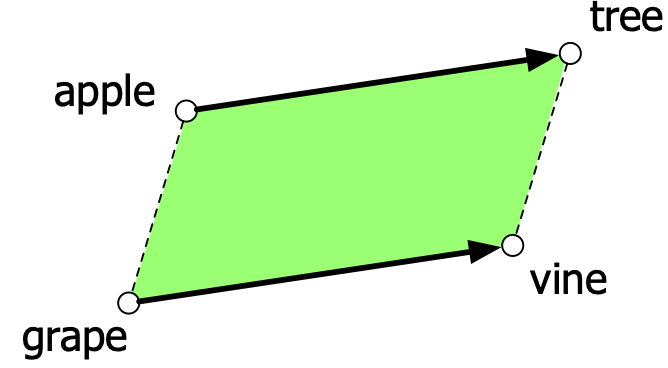
\includegraphics[height=3cm]{figures/analogy}
            \caption{Parallelogram model (from J\&H).}
        \end{figure}
        \vspace{-1em}
            \begin{itemize}
                \item man : woman :: king : queen
                \item[] $\phi_{\text{wrd}}(\text{man}) - \phi_{\text{wrd}}(\text{king}) \approx \phi_{\text{wrd}}(\text{woman}) - \phi_{\text{wrd}}(\text{queen})$
                %\item man : woman :: king : ? 
                %\item[] $\argmax_{w\in\sV} \text{sim}(-\phi_{\text{wrd}}(\text{man}) + \phi_{\text{wrd}}(\text{woman}) + \phi_{\text{wrd}}(\text{king}), w)$
                \item Caveat: must exclude the three input words
                \item Does not work for general relations
            \end{itemize}
            \pdfnote{
                While embedding spaces perform well if the task involves frequent words, small distances, and certain relations (like relating countries with their capitals or verbs/nouns with their inflected forms), the parallelogram method with embeddings doesn’t work as well for other relations
            }
\end{frame}

\begin{frame}
    {Comparison}
    \begin{table}
        \begin{tabular}{p{5cm}p{7cm}}
            Count-based & Prediction-based \\
            \midrule
            matrix factorization & prediction problem \\
            fast to compute & slow (with large corpus) but more flexible \\
            interpretable components & hard to interprete but has intriguing properties
        \end{tabular}

        \begin{itemize}
            \item Both uses the \textbf{distributional hypothesis}.
            \item Both generalize beyond text: using co-occurence between any types of objects
                \begin{itemize}
                    \item Learn product embeddings from customer orders
                    \item Learn region embeddings from images
                \end{itemize}
        \end{itemize}
    \end{table}
\end{frame}

\begin{frame}
    {Evaluate word vectors}
    \textbf{Intrinsic evaluation}\\
    \begin{itemize}
        \item Evaluate on the proxy task (related to the learning objective)
        \item Word similarity/analogy datasets (\eg WordSim-353, SimLex-999)
    \end{itemize}

    \textbf{Extrinsic evaluation}\\
    \begin{itemize}
        \item Evaluate on the real/downstream task we care about
        \item Use word vectors as features in NER, parsing etc.
    \end{itemize}
\end{frame}

\begin{frame}
    {Summary}
    \beamerblue{Key idea}: formalize word representation learning as a self-supervised prediction problem

    Prediction problems:\\
    \begin{itemize}
        \item Skip-gram: Predict context from words
        \item CBOW: Predict word from context
        \item Other possibilities:
            \begin{itemize}
                \item Predict $\log \hat{p} (\text{word}\mid \text{context})$, e.g. GloVe
                \item Contextual word embeddings (later)
            \end{itemize}
    \end{itemize}

\end{frame}


\section{Neural networks}

\begin{frame}
    {Feature learning}
    Linear predictor with handcrafted features: $f(x) = w\cdot\phi(x)$.

    Can we learn intermediate features?
    \pause

    Example:\\
    \begin{itemize}
    \item Predict popularity of restaurants.
    \item Raw input: \#dishes, price, wine option, zip code, \#seats, size 
    \item Decompose into subproblems:
    \begin{itemize}
        \itemsep2ex
    \item[] ${\color{blue}h_1}(\pb{\text{\#dishes, price, wine option}}) = \text{food quality}$
    \item[] ${\color{blue}h_2}(\pb{\text{zip code}}) = \text{walkable}$
    \item[] ${\color{blue}h_3}(\pb{\text{\#seats, size}}) = \text{nosie}$
    \end{itemize}
    \end{itemize}

\end{frame}

\begin{frame}
{Predefined subproblems}
\begin{center}
\def\layersep{2.5cm}
\begin{tikzpicture}[shorten >=1pt,->,draw=black!50, node distance=\layersep]
    \tikzstyle{every pin edge}=[<-,shorten <=1pt]
    \tikzstyle{neuron}=[circle,fill=black!25,minimum size=17pt,inner sep=0pt]
    \tikzstyle{input neuron}=[neuron, fill=green!50];
    \tikzstyle{output neuron}=[neuron, fill=red!50];
    \tikzstyle{hidden neuron}=[neuron, fill=blue!50];
    \tikzstyle{annot} = [text width=4em, text centered]

    % Draw the input layer nodes
    \foreach \name / \y / \text in {1/1/\#dishes, 2/2/price, 3/3/wine option, 4/4/zip code, 5/5/\#seats, 6/6/size}
    % This is the same as writing \foreach \name / \y in {1/1,2/2,3/3,4/4}
        \node[input neuron, pin=left:\text] (I-\name) at (0,-\y) {};

    % Draw the hidden layer nodes
    \foreach \name / \y in {1,...,3}
        \path[yshift=-1.3cm]
            node[hidden neuron] (H-\name) at (\layersep,-\y cm) {};

    % Draw the output layer node
    \node[output neuron,node distance=4cm,pin={[pin edge={->}]right:Popularity}, right of=H-2] (O) {};

    % Connect every node in the input layer with every node in the
    % hidden layer.
%    \foreach \source in {1,...,6}
%        \foreach \dest in {1,...,3}
%            \path (I-\source) edge (H-\dest);
	\foreach \source in {1,2,3}
		\path (I-\source) edge (H-1);
	\foreach \source in {4}
		\path (I-\source) edge (H-2);
	\foreach \source in {5,6}
		\path (I-\source) edge (H-3);

    % Connect every node in the hidden layer with the output layer
    \foreach \source in {1,...,3}
        \path (H-\source) edge (O);

    % Annotate the layers
    \node[annot,above of=H-1, node distance=2.5cm] (hl) {Intermediate features};
    \node[annot,left of=hl] {Input features};
    \node[annot,right of=hl, node distance=4cm] {Output};
    
    % Annotate the hidden nodes
    \foreach \h / \text in {1/food quality, 2/walkable, 3/noise}
    		\node[annot, above of=H-\h, node distance=0.5cm] {$h_\h$};
    \foreach \h / \text in {1/food quality, 2/walkable, 3/noise}
    		\node[annot, right of=H-\h, node distance=2cm, text width=4cm] {\text};
\end{tikzpicture}
\end{center}
\pdfnote{Let's try to represent our model as a graph. So we have nodes representing each input, nodes representing the intermediate predictors which takes in a subset of inputs, and the node representing the linear classifier that computes the output.}
\pdfnote{The subproblems are manually specified based on our knowledge of the problem. 
In fact, feature engineering is an important step when building practical ML models, but in this course so far we have ignored that part and assume they are given to use.
But we don't always have this knowledge, or our features aren't good, or we simply want to automate as many steps as possible.
It would be desirable if we can directly learn these subproblems.}
\end{frame}

\begin{frame}
    {Learning intermediate features}
\begin{center}
\def\layersep{2.5cm}
\begin{tikzpicture}[shorten >=1pt,->,draw=black!50, node distance=\layersep]
    \tikzstyle{every pin edge}=[<-,shorten <=1pt]
    \tikzstyle{neuron}=[circle,fill=black!25,minimum size=17pt,inner sep=0pt]
    \tikzstyle{input neuron}=[neuron, fill=green!50];
    \tikzstyle{output neuron}=[neuron, fill=red!50];
    \tikzstyle{hidden neuron}=[neuron, fill=blue!50];
    \tikzstyle{annot} = [text width=4em, text centered]

    % Draw the input layer nodes
    \foreach \name / \y / \text in {1/1/\#dishes, 2/2/price, 3/3/wine option, 4/4/zip code, 5/5/\#seats, 6/6/size}
    % This is the same as writing \foreach \name / \y in {1/1,2/2,3/3,4/4}
        \node[input neuron, pin=left:\text] (I-\name) at (0,-\y) {};

    % Draw the hidden layer nodes
    \foreach \name / \y in {1,...,3}
        \path[yshift=-1.3cm]
            node[hidden neuron] (H-\name) at (\layersep,-\y cm) {};

    % Draw the output layer node
    \node[output neuron,node distance=4cm,pin={[pin edge={->}]right:Popularity}, right of=H-2] (O) {};

    % Connect every node in the input layer with every node in the
    % hidden layer.
    \foreach \source in {1,...,6}
        \foreach \dest in {1,...,3}
            \path (I-\source) edge (H-\dest);

    % Connect every node in the hidden layer with the output layer
    \foreach \source in {1,...,3}
        \path (H-\source) edge (O);

    % Annotate the layers
    \node[annot,above of=H-1, node distance=2.5cm] (hl) {\textcolor{blue}{Hidden} layer};
    \node[annot,left of=hl] {Input layer};
    \node[annot,right of=hl, node distance=4cm] {Output layer};
    
    % Annotate the hidden nodes
    \foreach \h / \text in {1/food quality, 2/walkable, 3/noise}
    		\node[annot, above of=H-\h, node distance=0.5cm] {$h_\h$};
\end{tikzpicture}
\end{center}
\end{frame}

\begin{frame}
    {Neural networks}
\beamerblue{Key idea}: automatically learn the intermediate features.

    \textbf{Feature engineering}:
Manually specify $\phi(x)$ based on domain knowledge and learn the weights:
\begin{align*}
f(x) = {\color{red}w}^T\phi(x) .
\end{align*}

    \textbf{Feature learning}:
Automatically learn both the features ($K$ hidden units) and the weights:
\begin{align*}
h(x) = \pb{{\color{red}h_1}(x), \ldots, {\color{red}h_K}(x)} , \quad
f(x) = {\color{red}w}^T h(x)
\end{align*}
\end{frame}

\begin{frame}
{Activation function}
\begin{itemize}[<+->]
\item How should we parametrize $h_i$'s? Can it be linear?
\onslide<+->{
\begin{align}
h_i(x) = {\color{blue}\sigma}(v_i^T x) .
\end{align}
}
\item<.-> $\sigma$ is the \emph{nonlinear} \textbf{activation function}.
\item What might be some activation functions we want to use?
\begin{itemize}
\item $\text{sign}$ function? \red{Non-differentiable}.
\item \emph{Differentiable} approximations: sigmoid functions.
\begin{itemize}[<.->]
\item E.g., logistic function, hyperbolic tangent function, ReLU
\end{itemize}
\end{itemize}
\item Two-layer neural network (one \textcolor{blue}{hidden layer} and one  \textcolor{Green}{output layer}) with $K$ hidden units:
\begin{align}
f(x) &= \sum_{k=1}^{K} {\color{Green}w_k} h_k(x) = \sum_{k=1}^K {\color{Green}w_k} \sigma({\color{blue}v_k}^T x)
\end{align}
\end{itemize}
\pdfnote{Recall that $h$ is an intermediate predictor. How about the sign function such that $h$ would output the result of a binary classifier.}
\pdfnote{Sigmoid function is S-shaped functions that approximate sign function. (draw)}
\pdfnote{Let's write down our two-layer network. In the output layer, we have a linear combination of the hidden units. Each hidden units compute a linear combination of its inputs followed by an activation function.}
\pdfnote{Without the activation function this is just a linear model. What do we gain from these nonlinear activation functions? Let's look at how well a two layer NN approximate different functions.}
\end{frame}

\begin{frame}{Activation Functions}

\begin{itemize}
\item The \textbf{hyperbolic tangent} is a common activation function:
\[
\sigma(x)=\tanh\left(x\right).
\]
\end{itemize}
\begin{figure}
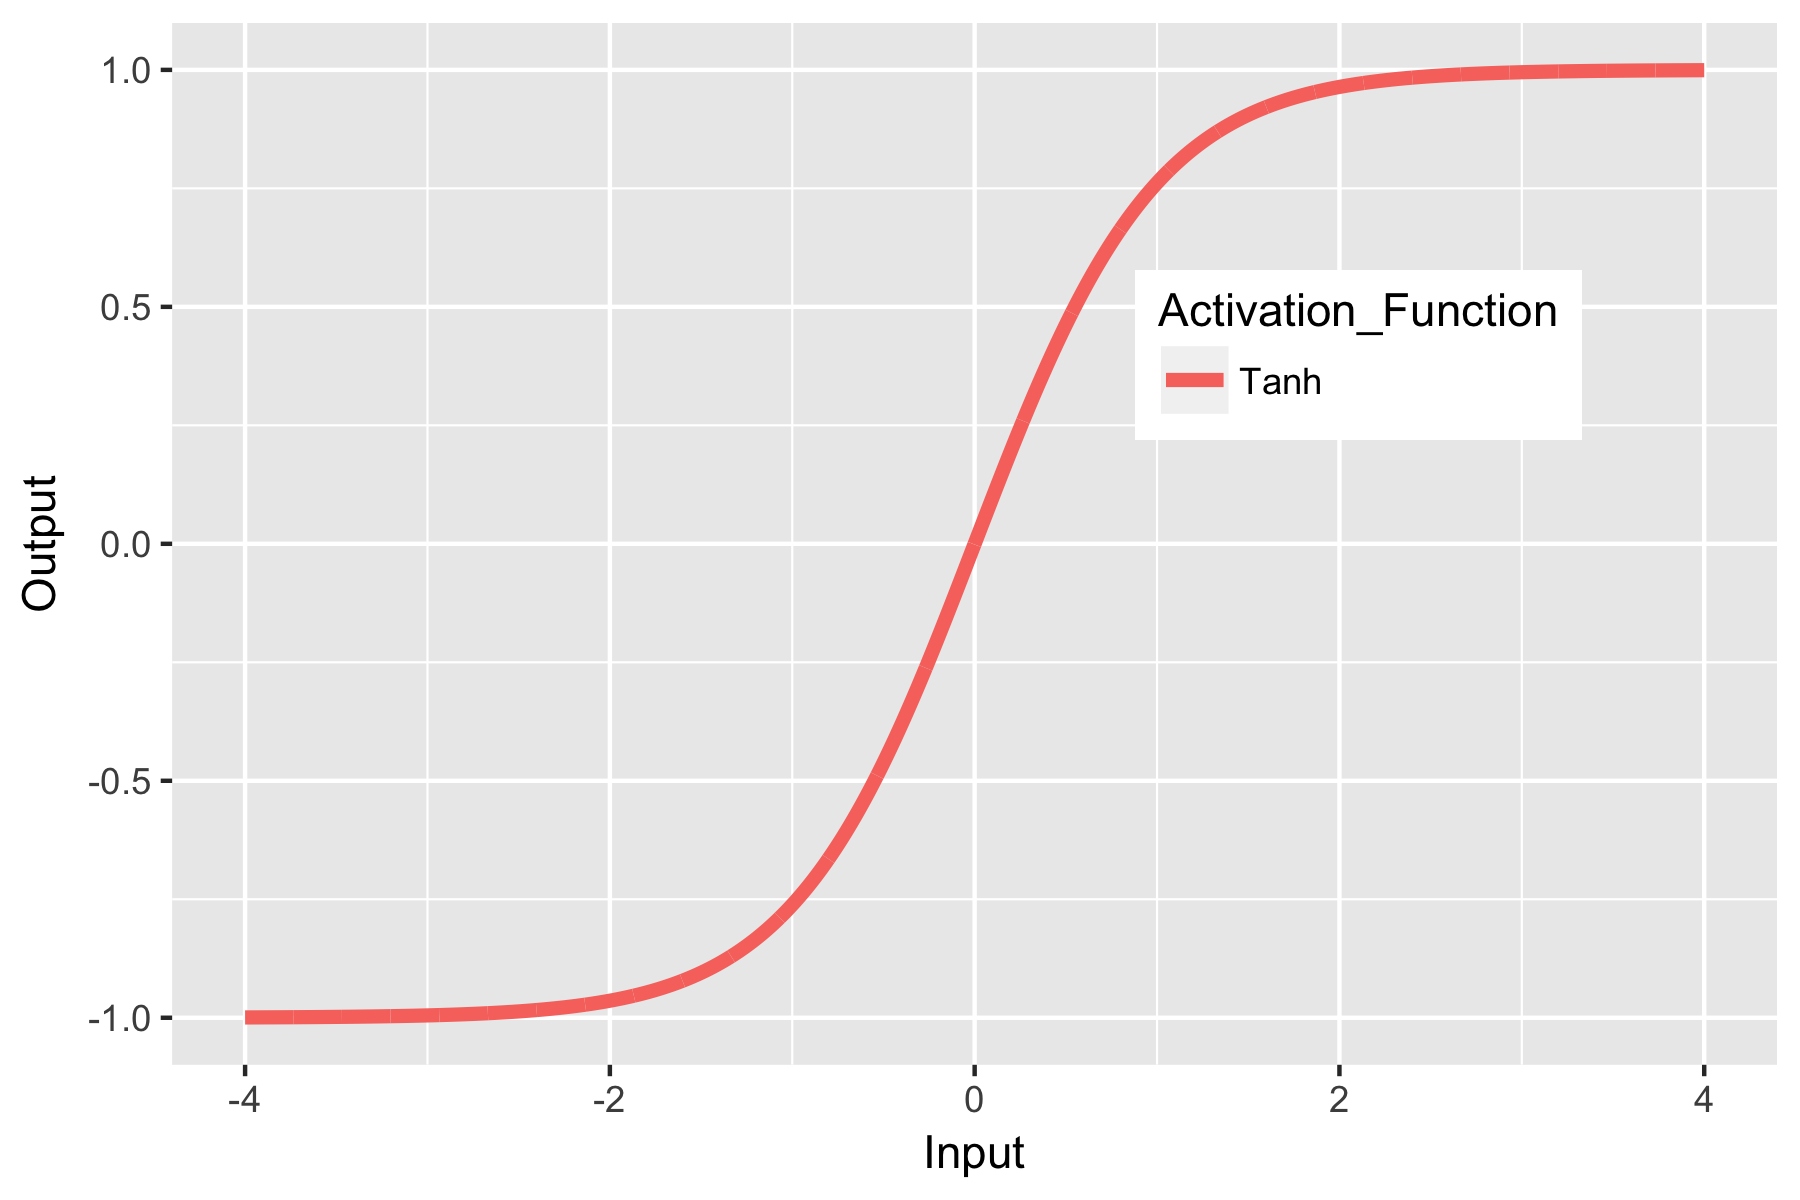
\includegraphics[height=0.55\textheight]{figures/activationFn-Tanh}
\end{figure}
\end{frame}
%
\begin{frame}{Activation Functions}
\begin{itemize}
\item More recently, the \textbf{rectified linear} (\textbf{ReLU}) function has been very
popular:
\[
\sigma(x)=\max(0,x).
\]
\item Much \textcolor{Green}{faster} to calculate, and to calculate
its derivatives.
\item Work well empirically.
\end{itemize}
\begin{figure}
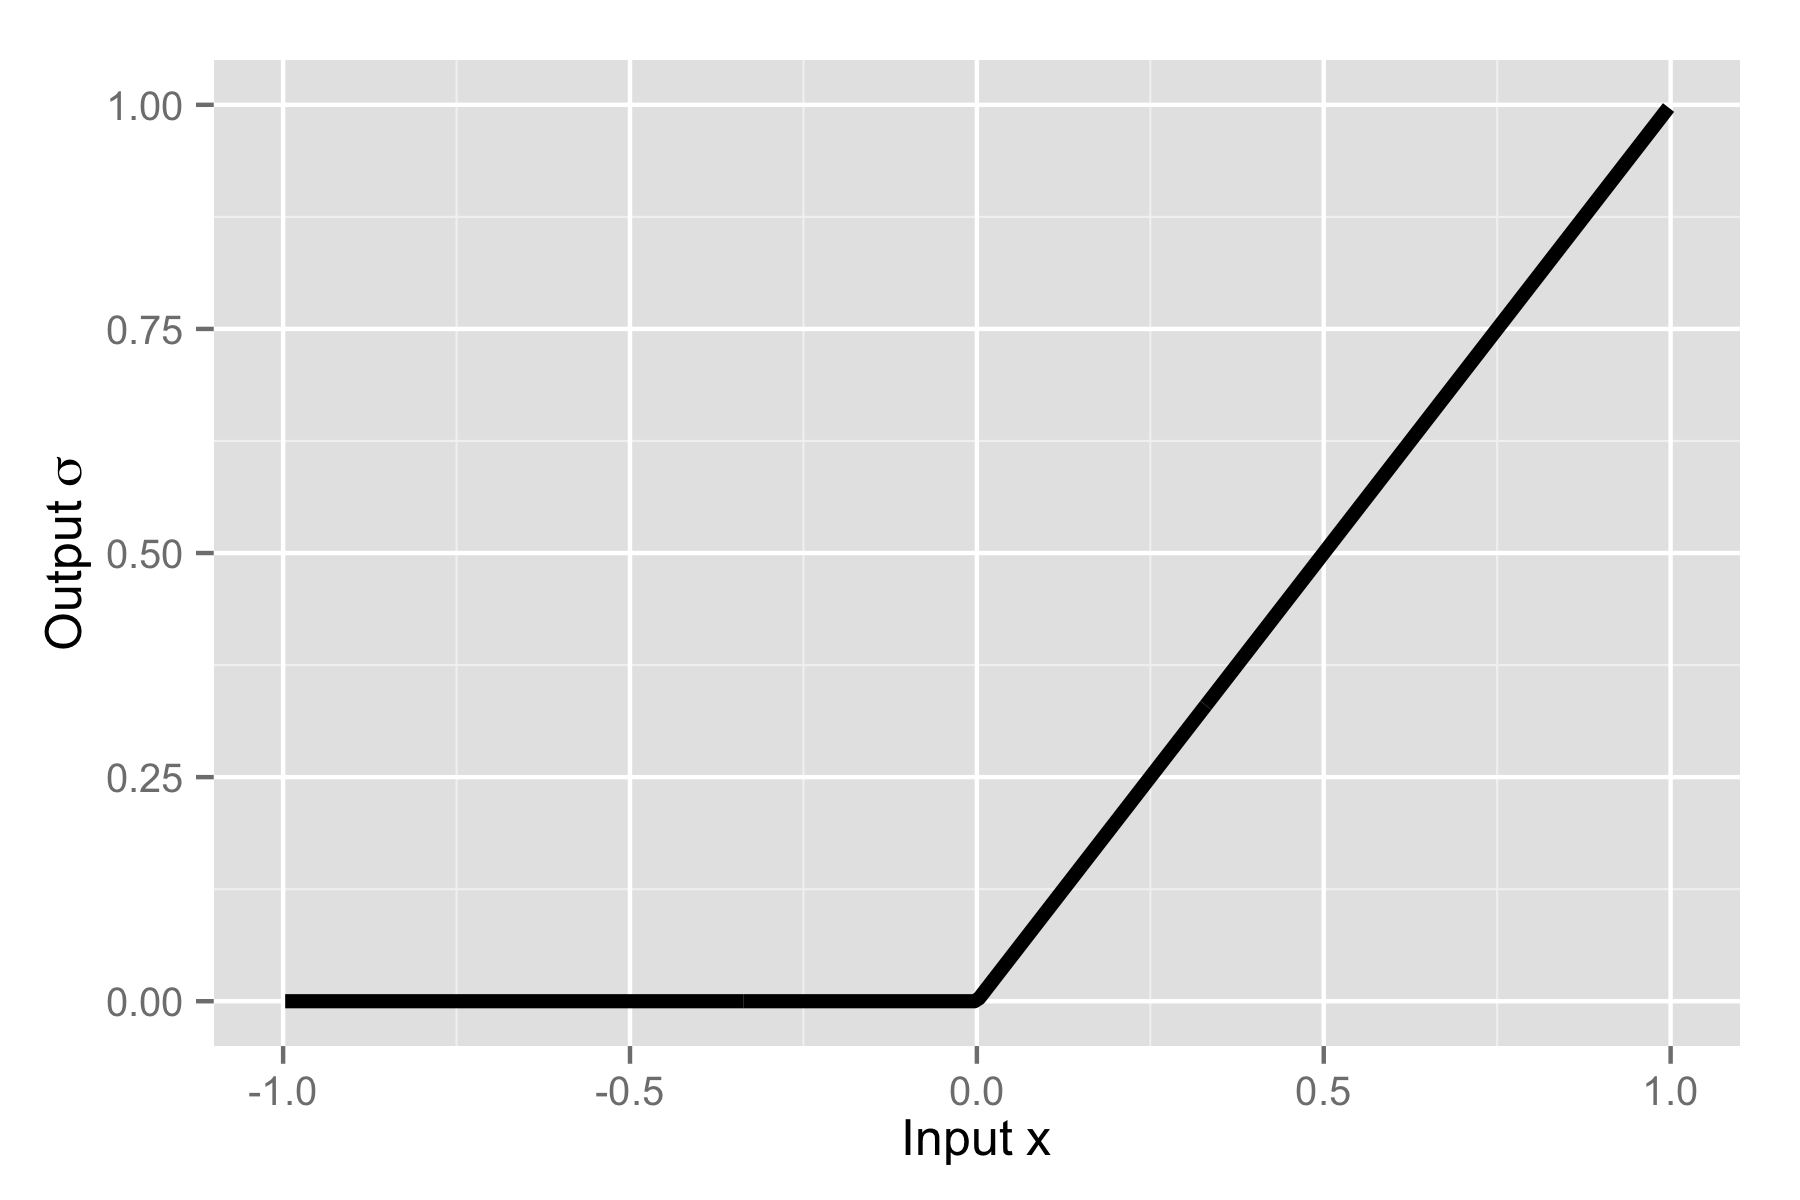
\includegraphics[height=0.55\textheight]{figures/activationFn-Rectified_Linear} 
\end{figure}
\end{frame}

\begin{frame}
{Multilayer perceptron / Feed-forward neural networks}
\begin{itemize}
\item Wider: more hidden units.
\item Deeper: more hidden layers.
\end{itemize}
\begin{center}
\def\layersep{2.5cm}
\begin{tikzpicture}[shorten >=1pt,->,draw=black!50, node distance=\layersep]
    \tikzstyle{every pin edge}=[<-,shorten <=1pt]
    \tikzstyle{neuron}=[circle,fill=black!25,minimum size=17pt,inner sep=0pt]
    \tikzstyle{input neuron}=[neuron, fill=green!50];
    \tikzstyle{output neuron}=[neuron, fill=red!50];
    \tikzstyle{hidden neuron}=[neuron, fill=blue!50];
    \tikzstyle{annot} = [text width=4em, text centered]

    % Draw the input layer nodes
    \foreach \name / \y / \text in {1/1/1, 2/2/2, 3/3/, 4/4/d-1, 5/5/d}{
    		\ifthenelse{\y=3}
    		{\node[input neuron, pin=left:$\vdots$] (I-\name) at (0,-\y) {}}
        {\node[input neuron, pin=left:$x_{\text}$] (I-\name) at (0,-\y) {}}
	;}
    % Draw the hidden layer nodes
    \foreach \name / \y in {1,...,4}
        \path[yshift=-.5cm]
            node[hidden neuron] (H-\name) at (\layersep,-\y cm) {};
            
    % Draw the hidden layer nodes
    \foreach \name / \y in {1,...,3}
        \path[yshift=-1cm]
            node[hidden neuron] (H2-\name) at (2*\layersep,-\y cm) {};

    % Draw the output layer node
    \node[output neuron,pin={[pin edge={->}]right:score}, right of=H2-2] (O) {};

    % Connect every node in the input layer with every node in the
    % hidden layer.
    \foreach \source in {1,...,5}
        \foreach \dest in {1,...,4}
            \path (I-\source) edge (H-\dest);
    \foreach \source in {1,...,4}
        \foreach \dest in {1,...,3}
            \path (H-\source) edge (H2-\dest);

    % Connect every node in the hidden layer with the output layer
    \foreach \source in {1,...,3}
        \path (H2-\source) edge (O);

    % Annotate the layers
    \node[annot,above of=H-1, node distance=1.3cm] (hl) {{Hidden} layers};
    \node[annot,left of=hl] {Input layer};
    \node[annot,right of=hl, node distance=5cm] {Output layer};
    
\end{tikzpicture}
\end{center}
\pdfnote{It's pretty easy to extend the two layer NN we just talked about. We can either add more hidden layers, or more hidden units in each layer. Modern neural networks usually have many hidden layers. If the nodes in any two adjacent layers are fully connected, we call it a MLP or FFNN.}
\end{frame}

\begin{frame}{Multilayer Perceptron: Standard Recipe}
\begin{itemize}[<+->]
\item Each subsequent hidden layer takes the \blue{output $o\in\BR^{m}$ of
previous layer} and produces
\[
h^{(j)}({\color{blue}o^{(j-1)}})=\sigma\left(W^{(j)}{\color{blue}o^{(j-1)}}+b^{(j)}\right),\text{ for }j=2,\ldots,L
\]
where $W^{(j)}\in\BR^{m\times m}$, $b^{(j)}\in\BR^{m}$.

\item Last layer is an \emph{affine} mapping (no activation function): 
\[
a(o^{(L)})=W^{(L+1)}o^{(L)}+b^{(L+1)},
\]
where $W^{(L+1)}\in\BR^{k\times m}$ and $b^{(L+1)}\in\BR^{k}$.

\item The full neural network function is given by the \emph{composition} of
layers:
\begin{align}
f(x) &= \left(a\circ h^{(L)}\circ\cdots\circ h^{(1)}\right)(x)
\end{align}

\item Last layer typically gives us a score. (How to do classification?)
\end{itemize}
\end{frame}

\end{document}
